%%% PREAMBLE - Do not touch %%%%%%%%%%%%%%%%%%%%%%%%%%%%%%%%%%%%%%%%%%%%%%%%%%%%%%
\documentclass[10pt,twocolumn,letterpaper]{article}
%%\usepackage[ansinew]{inputenc}
\usepackage[latin1,utf8]{inputenc}
\usepackage[portuges,brazil,english]{babel}
\usepackage{model}
\usepackage{times}
\usepackage{epsfig}
\usepackage{graphicx}
\usepackage{amsmath}
\usepackage{amssymb}
\usepackage{color}
\usepackage[pagebackref=true,breaklinks=true,letterpaper=true,colorlinks,bookmarks=false]{hyperref}
\usepackage{appendix}
%  ABACO -- Conjunto de macros para desenhar o 'abaco

%  Desenho original de Hans Liesenberg

%  Macros de Tomasz Kowaltowski

%  DCC -- IMECC -- UNICAMP

%  Mar,co de 1988  --  Vers~ao 1.0

% Ajustado para LaTeX da SUN -- Mar,co de 1991

% ---------------------------------------------------------

%  Chamada:   \ABACO{d1}{d2}{d3}{d4}{esc}
%             com:  di's -- os quatro d'igitos;
%	           esc  -- fator de escala

% ---------------------------------------------------------

%  DEFINI,C~OES AUXILIARES

% ---------------------------------------------------------


%  Forma o d'igito pequeno (0 ou 1)

\newcommand{\ABACODP}[1]{%
%
\thicklines
%    
\begin{picture}(8,0)
    \ifcase#1{   %  caso 0
       \put(0,0)    {\line(1,0){4}}
       \multiput(5,0)(2,0){2}{\oval(2,4)}}
    \or{         %  caso 1
       \put(2,0)    {\line(1,0){4}}
       \multiput(1,0)(6,0){2}{\oval(2,4)}}
    \fi
\end{picture}
    } % \ABACODP

% Forma o d'igito grande (0 a 4)

\newcommand{\ABACODG}[1]{%
%
\thicklines
%    
\begin{picture}(14,0)
    \ifcase#1{   % caso 0
       \multiput(1,0)(2,0){5}{\oval(2,4)}}
       \put(10,0)   {\line(1,0){4}}
    \or{         % caso 1
       \multiput(1,0)(2,0){4}{\oval(2,4)}}
       \put(8,0)   {\line(1,0){4}}
       \put(13,0)   {\oval(2,4)}
    \or{         % caso 2
       \multiput(1,0)(2,0){3}{\oval(2,4)}
       \put(6,0)   {\line(1,0){4}}
       \multiput(11,0)(2,0){2}{\oval(2,4)}}
    \or{         % caso 3
       \multiput(1,0)(2,0){2}{\oval(2,4)}
       \put(4,0)   {\line(1,0){4}}
       \multiput(9,0)(2,0){3}{\oval(2,4)}}
    \or{         % caso 4
       \put(1,0)  {\oval(2,4)}}
       \put(2,0)   {\line(1,0){4}}
       \multiput(7,0)(2,0){4}{\oval(2,4)}
    \fi
\end{picture}
    } % \ABACODG
       
% Forma um d'igito (0 a 9)

\newcommand{\ABACOD}[1]{%
%
    \ifnum#1>9
       \errmessage{#1: Argumento invalido para ABACO}
    \fi
    \ifnum#1<0
       \errmessage{#1: Argumento invalido para ABACO}
    \fi
%
\begin{picture}(24,0)
%    
    \ifnum#1<5
       \put(16,0) {\ABACODP{0}}
    \else   
       \put(16,0) {\ABACODP{1}}
    \fi
%    
    \ifnum#1<5
       \put(0,0)  {\ABACODG{#1}}
    \else
       \ifcase#1\or \or \or \or
          \or  \put(0,0)  {\ABACODG{0}}
          \or  \put(0,0)  {\ABACODG{1}}
          \or  \put(0,0)  {\ABACODG{2}}
          \or  \put(0,0)  {\ABACODG{3}}
          \or  \put(0,0)  {\ABACODG{4}}
       \fi
    \fi   
\end{picture}
    } % \ABACOD
    
% -------------------------------------------------

%  DEFINI,C~AO PRINCIPAL
    
\newcommand{\ABACO}[5]{%
    \setlength{\unitlength}{#5mm}
%
    \thinlines
%   
\begin{picture}(28,25)
%   
% moldura
%
% externa
%
        \put(0,0)            {\line(0,1){25}}
        \put(0,0)            {\line(1,0){28}}
        \put(28,0)           {\line(0,1){25}}
        \put(0,25)           {\line(1,0){28}}
% interna
        \put(2,2)            {\line(0,1){21}}
	\put(26,2)           {\line(0,1){21}}
	\put(16,2)           {\line(0,1){21}}
	\put(18,2)           {\line(0,1){21}}
	\put(2,2)            {\line(1,0){14}}
	\put(16,2)           {\line(1,-1){1}}
	\put(17,1)           {\line(1,1){1}}
	\put(18,2)           {\line(1,0){8}}
	\put(2,23)           {\line(1,0){14}}
	\put(16,23)          {\line(1,1){1}}
	\put(17,24)          {\line(1,-1){1}}
	\put(18,23)          {\line(1,0){8}}
	\put(0,0)            {\line(1,1){2}}
	\put(0,25)           {\line(1,-1){2}}
	\put(28,0)           {\line(-1,1){2}}
	\put(28,25)          {\line(-1,-1){2}}
%
%   
% d'igitos
%
%   
       \put(2,20)  {\ABACOD{#1}}
       \put(2,15)  {\ABACOD{#2}}
       \put(2,10)  {\ABACOD{#3}}
       \put(2,5)   {\ABACOD{#4}}
%      
\end{picture}
    } % \ABACO
    


\cvprfinalcopy % *** Uncomment this line for the final submission
\def\httilde{\mbox{\tt\raisebox{-.5ex}{\symbol{126}}}}
\ifcvprfinal\pagestyle{empty}\fi

\newcommand{\TODO}[1]{TODO: #1}
\newcommand{\CITEONE}[2]{\mbox{#1 \cite{#2}}}
\newcommand{\CITETWO}[3]{\mbox{#1 and #2 \cite{#3}}}
\newcommand{\CITEN}[2]{\mbox{#1 et al. \cite{#2}}}

%%% Paper beginning %%%%%%%%%%%%%%%%%%%%%%%%%%%%%%%%%%%%%%%%%%%%%%%%%%%%%%%%%%%%%%
\begin{document}

%%% Title and authors %%%%%%%%%%%%%%%%%%%%%%%%%%%%%%%%%%%%%%%%%%%%%%%%%%%%%%%%%%%%
\title{Printer ballistics through texture analysis of characters}
\author{Adriano Ruggero\thanks{Institute of Computing, University of Campinas (Unicamp). \textbf{Contact}: \tt\small{arruggero@lasca.ic.unicamp.br}}\\
Gabriel Rodrigues\thanks{Institute of Computing, University of Campinas (Unicamp). \textbf{Contact}: \tt\small{gabriel\_rodrigues@aol.com}}\\
Mário Brito\thanks{Institute of Computing, University of Campinas (Unicamp). \textbf{Contact}:
\tt\small{britomar@aedu.com}}\\
Maurício Perez\thanks{Institute of Computing, University of Campinas (Unicamp). \textbf{Contact}:
\tt\small{mauriciolp84@gmail.com}}\\
Anderson Rocha\thanks{Institute of Computing, University of Campinas (Unicamp). \textbf{Contact}: \tt\small{anderson.rocha@ic.unicamp.br}}
}

%%% Abstract %%%%%%%%%%%%%%%%%%%%%%%%%%%%%%%%%%%%%%%%%%%%%%%%%%%%%%%%%%%%%%%%%%%%%
\maketitle
\begin{abstract}
We describe a technique for ballistics of printed documents, that is, link a printed document to a specific printer. The principle of this technique is the analysis of character's texture, by extracting some properties from the characters of scanned images from the printed documents, and relate this properties through a co-occurrence matrix. This matrix can be used to create a "fingerprint" for the characters related to the same printer, what allows us to identify the specific printer device that printed these characters.
\end{abstract}

%%% Introduction %%%%%%%%%%%%%%%%%%%%%%%%%%%%%%%%%%%%%%%%%%%%%%%%%%%%%%%%%%%%%%%%%
\section{Introduction}
\label{sec:introduction}

In August of 2013, a russian man wrote his own small print in a credit card contract~\cite{RT}. The credit card's administrator bank didn't read the amendments made by the client, and just signed and certified the document. The changes included unlimited credit line, 0 percent interest rates and no fees. When the bank decided to terminate the man's credit card, because overdue payments, he sued them for more than 24 million rubles (US\$ 727.000). How could the bank prove the falsification?

Altough we are living in a digital era, printed documents still are a significant part of our day by day. Likewise, with the constant reduction in prices and increase in quality of printing equipment, forgeries become increasingly commonplace.

Legal aspects aside, a way to verify if a document, or a part of it, came from a specific device can be through  character's texture analysis.

Our approach for the analysis of character's texture is as follows. From printed pages scanned at high resolution, selected characters were extracted. From these characters, we obtained its properties of contrast, correlation, energy and homogeneity, creating with them a co-occurrence matrix. This matrix can be called a ''fingerprint'' of the character. This ''fingerprint'' of  characters is closely related to the printing device which originated it, and can be used to identify which printer was responsible for printing it.

However, slight imperfections may occur during the printing and/or scanning process of documents. To handle these small errors (or variations), characters were selected from different areas of scanned document, their properties were obtained and then classified using machine learning algorithms.

%%% Add section %%%%%%%%%%%%%%%%%%%%%%%%%%%%%%%%%%%%%%%%%%%%%%%%%%%%%%%%%%%%%%%%%%
\section{State-of-the-Art}
\label{sec:state_of_the_art}

Literature on the identification of printing devices from their printed documents is not wide in Academia. The work of Kee and Farid \cite{Printer_Profiling} reports a technique of geometric modeling of degradation caused by the printer. According to the authors, this degradation, measured based on a character basis, is modeled constructing a linear basis from characters commonly found on a printed page. From the point of view of ballistics, the accuracy of the developed technique allows to identify the device that originated the printed pages. According to the authors, the technique allows to distinguish between printers of different brands and models, but not among printers of the same make and model.

The work Bulan et al \cite{Bulan} demonstrates a technique for analyzing geometric distortions introduced during the printing process of electrophotographic printers (EP). According to the authors, it is first determined the geometric distortion signature to the printer using only printed pages. It is then built up a database and the printer used to print a test page is identified by computing the geometric distortion signature from the printed test page and correlated it with the signatures present in the database. Geometric distortion signature is calculated comparing dot positions extracted from the printed image and estimated dot positions before printing.

The work of Pollard et al \cite{Pollard} presents a general method for extracting a signature print from the outer boundary of a text glyph.

Valuable is also the work of Rocha and Leite \cite{Rocha}. This work deals with the concept of analysis of textures through co-occurrence matrix, used as a cornerstone of the solution proposed by us.

%%% Add section %%%%%%%%%%%%%%%%%%%%%%%%%%%%%%%%%%%%%%%%%%%%%%%%%%%%%%%%%%%%%%%%%%
\section{Proposed Solution}
\label{sec:proposed_solution}

Our solution consist in getting the image of characters selected from scanned documents in grayscale, extract its properties of contrast, correlation, energy and homogeneity - creating a co-occurrence matrix - and cluster them by machine learning algorithms.

\subsection{Printers dataset}
\label{subsec:printers_dataset}

The documents used for this work were obtained from the Wikipedia site~\cite{Wikipedia}, and were written in English, some of them containing pictures, some not. They were printed by printers listed in Table \ref{tab:printers}. 






\begin{table*}
\caption{Printers used in this work}
\label{tab:printers}
\begin{center}
    \begin{tabular}{ | c | c | c | c |}
    \hline
Printer & Documents & Characters ''e'' & Characters ''t'' \\ \hline
Brother-HL4070CDW & 28 & 252 & 252\\
Canon-D1150 & 28 & 252 & 252\\
Canon-MF3240 & 28 & 252 & 252\\
Canon-MF4370DN & 27 & 252 & 252 \\
HP-CLJ-CP2025A & 28 & 250 & 250\\
Lexmark-E260D & 30 & 636 & 629\\
\hline
    \end{tabular}
\end{center}    
\end{table*}

These printed documents were scanned at high resolution and saved as Tiff file format (Tagged Image File Format), forming a database. These files were made available through an FTP site~\cite{Printers_dataset}. An example of a typical document used in this study can be seen in Figure \ref{fig:document}.

\begin{figure}
\begin{center}
	\includegraphics[width=0.99\columnwidth]{document}
	\caption{Typical document used in this work~\cite{Wikipedia}.}
\label{fig:document}   
\end{center} 
\end{figure}

\subsection{Characters}
\label{subsec:characters}

The characters chosen for this work were "e" and "t", both in lowercase, because they are, respectively, the first and second most common letters in texts written in English~\cite{Letter_Frequency}.

To avoid inconsistencies and / or values "off the curve", we used only characters printed in the same font and size, for all printers. With the same objective, we used only characters printed in normal font, not analyzing characters in bold, italic, underline, strikeout, superscript, subscript, or any other form of letter change.

Were not considered characters from misaligned documents, i.e. characters from apparently obliquely scanned documents. Figure \ref{fig:characters} shows examples of two characters obtained from scanned documents, one of them being usable and the other not, being considered rotated.

\begin{figure}
\begin{center}
	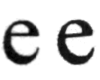
\includegraphics[width=0.99\columnwidth]{characters}
	\caption{Examples of characters: the left one was considered useful; the right one, slightly rotated.}
\label{fig:characters}   
\end{center} 
\end{figure}

Subsection \ref{subsec:co-occurence_matrix} will be explained in more detail why not use rotated characters.

\subsection{Printers}
\label{subsec:printers}

Due to the fact that all scanned documents come from laser printers, it was necessary to take some precautionary measures. Laser printers are known as ''page printers'', while dot matrix printers and inkjet printers are called ''line printers''. This is a crucial difference, and should be considered for more careful study. 

Line printers print documents line by line from the top of the sheet, keeping a characteristic pattern which periodically repeats for each paper feed. That is, any line printed by this printer model will have basically the same characteristics, regardless of their vertical location in the paper sheet. 

Page printers, instead, do not print documents line by line. In this case, an image of the entire page is ''printed'' on the photoreceptor drum by a laser unit. This image attracts toner particles, and then transfers it to the paper sheet. Finally, a fuser unit heats the paper, so the toner melts and attach it. Figure \ref{fig:page_printer} shows a default page printer schema.

\begin{figure}
\begin{center}
	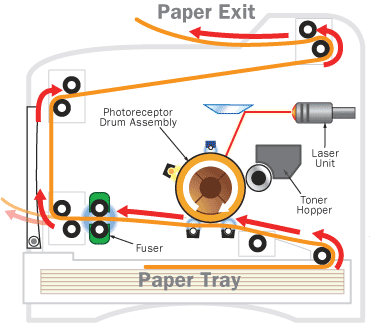
\includegraphics[width=0.99\columnwidth]{page_printer}
	\caption{Default page printer schema~\cite{Document_Analysis}.}
\label{fig:page_printer}   
\end{center} 
\end{figure}

By working in this way, page printers do not maintain a characteristic pattern that is repeated line by line across the printed paper sheet. Due to small imperfections that may exist in the photoreceptor drum, each print area generated by this type of device can present different characteristics.
Taking into account this fact, it was necessary to obtain characters from different parts of the scanned document. 

Basically, each document has roughly divided into three parts: upper, middle, and bottom. The Figure \ref{fig:document_areas} shows an example of a document divided in this way. If this article is being viewed in color, the upper part of the figure is in red, the middle, in green and bottom, in blue.

\begin{figure}
\begin{center}
	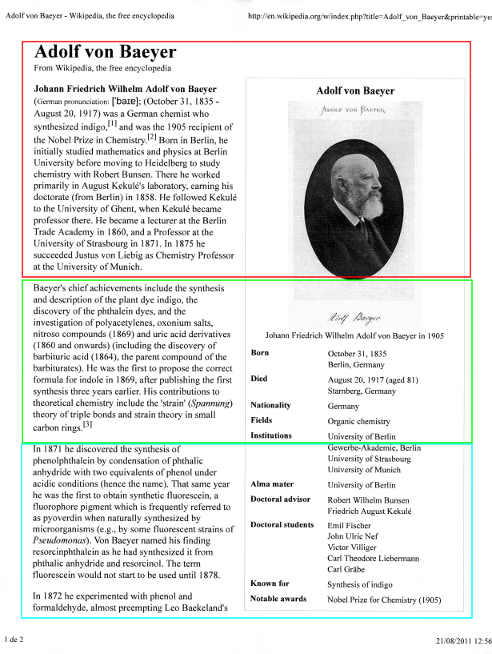
\includegraphics[width=0.99\columnwidth]{document_areas}
	\caption{Division of the scanned document in areas.}
\label{fig:document_areas}   
\end{center} 
\end{figure}

Despite showing subtle differences between characters located in different areas of the printout, the print device maintains certain intrinsic characteristics unchanged in all printed characters. Such characteristics can be compared to our fingerprints, making it a way to link a printed character to a particular device.

\subsection{Gray level co-occurence matrix}
\label{subsec:co-occurence_matrix}

Co-occurrence matrix is a tabulation of how many different combinations of intensity values of pixels (grayscale) occur in an image. The primary use of the co-occurrence matrix is characterized texture in an image from a set of statistics for instances of
each gray level in different pixels along different directions~\cite{Rocha}.

Co-occurrence matrix considers the relationship between two pixels at a time, one called as ''reference pixel'' and another as ''neighbor pixel''. The neighboring pixel chosen can be neighbor in any direction: east (right), west (left), north (above), south (below), or diagonally, i.e. northeast, northwest, southwest and southeast of each reference pixel. Also the neighborhood need not be exactly one pixel, can be 2, 3, or any value. Each pixel within the image becomes the reference pixel, starting at the top left and proceeding to the lower right. There will be particular cases. For instance, pixels of the right margin of the image does not have neighboring right.

Co-occurrence, in its most general form, can be specified by a matrix of relative frequencies $P (i, j, d,\theta)$, where two neighboring texture elements separated by a distance $d$ in a direction $\theta$ occur in the image, one with the property $i$ and another with property $j$.

From a co-occurrence matrix can be obtained some properties of the analyzed image. For this work, we used the properties of contrast, correlation, energy and homogeneity to create a fingerprint of the printed characters.

Using an example similar to the rotated character, we can compare the value differences in the properties obtained from the co-occurrence matrix (Figure \ref{fig:characters_angle}). In this case, the character on the left was obtained directly from the scanned document; character on the right is the same character, but rotated -4º.

\begin{figure}
\begin{center}
	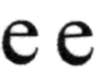
\includegraphics[width=0.99\columnwidth]{characters_angle}
	\caption{On the left, a character obtained from a scanned document and to the right, the same character, rotated -4º.}
\label{fig:characters_angle}   
\end{center} 
\end{figure}

Table \ref{tab:properties_differences} lists the differences between the properties of the character sample obtained from the co-occurrence matrix.

\begin{table}
\label{tab:properties_differences}
\caption{Differences between an original character and a rotated character.}
\begin{center}
\begin{tabular}{l*{3}{c}r}
Property & Original character & Rotated character (-4º) \\
\hline
Contrast & 3.2443 - 2.2905 & 5.1617 - 4.6504 \\
Correlation & 0.7869 - 0.8502 & 0.6967 - 0.7264 \\
Energy & 0.1608 - 0.1744 & 0.1106 - 0.1216 \\
Homogeneity & 0.6946 - 0.7462 & 0.6610 - 0.6995 \\
\end{tabular}
\end{center}
\end{table}

As shown in the Table \ref{tab:properties_differences}, small changes in the alignment of the print / scan can cause large variations in the properties values obtained from the co-occurrence matrix.

Details on how to calculate values of contrast, correlation, energy and homogeneity can be seen in Appendix A.

%%% Add section %%%%%%%%%%%%%%%%%%%%%%%%%%%%%%%%%%%%%%%%%%%%%%%%%%%%%%%%%%%%%%%%%%
\section{Experiments and Discussion}
\label{sec:experiments}

As a starting point for our experiments, it was necessary to select the desired characters from the documents on which the proprieties would be extracted. With the extracted proprieties of contrast, correlation, energy and homogeneity from the characters, we started evaluating the best methodology and machine learning algorithms for our solution. In the first instance, we needed to determine the best options for classifying the characters and attributing them to a Printer. But our final goal is not to attribute the characters to a printer, but a whole document, so in the next step, we propose a way of attributing the printer based on the classification of the characters.

\subsection{Characters Selection and Proprieties Extraction}

First we selected three characters from each one of the three sections from a document, and repeated that for all documents. There were 3x3x28 = 252 characters selected for each printer, what gave us a total of 1512.

For the proprieties extraction we used two different neighborhoods show in figure \ref{fig:neighbor}. From the first neighborhood we gathered two characteristics per type (contrast, correlation, energy and homogeneity), originating a vector of descriptors of eight values for a character. The second one gave us four per type, in other words, a sixteen sized vector.

\begin{figure}
\begin{center}
	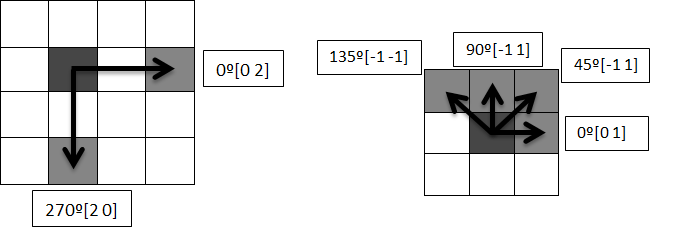
\includegraphics[width=0.99\columnwidth]{neighbor}
	\caption{Neighborhood A, leftmost, and B, rightmost, used in properties extraction (the darker pixel is the pixel-of-interest).}
\label{fig:neighbor}   
\end{center} 
\end{figure}

\subsection{Characters Classification}

The just acquired descriptors are used for evaluation the available classification algorithms. For this evaluation it was separated 66\% of the chars to be used as training (1008) and the rest for testing (504). From them we separate the most prominent and present the results in table \ref{tab:correct_classification}.

\begin{table}
\label{tab:correct_classification}
\caption{Percentage of correct classifications of printers.}
\begin{center}
\begin{small} 
\setlength{\tabcolsep}{3pt} 
\begin{tabular}{l*{5}{c}r} & \multicolumn{2}{c}{Neighborhood A} & \multicolumn{2}{c}{Neighborhood B}\\ \cline{1-5}
Method & Chars e’s & Chars t’s & Chars e’s & Chars t’s \\
\hline
Logistic & 81 & 81.3 & 85 & 84.6\\
KStar & 77.6 & 83 & 72 & 79.6\\
RotationForest & 83.1 & 85 & 81.7 & 85.7\\
NNge & 74.1 & 80.2 & 72.2 & 67.8\\
LMT & 83.8 & 84.6 & 82.7 & 85.5\\

\end{tabular}
\end{small}
\end{center}
\end{table}

Analyzing the results we can see a slightly better classification on the characters ''t'', perhaps they are more unique for each printer. The results also show that using a neighborhood of four pixels for many cases made the classification worst, what was against our intuition since its descriptors were longer than of the other neighborhood we used.

\subsection{Printer Attribution}

As said before, attributing a printer to the character is not the main objective, so it was necessary to define a logical output from the classified characters obtained in the previous step. For this purpose we choose to attribute a document to the printer that had most classified characters on it.

%%% Add section %%%%%%%%%%%%%%%%%%%%%%%%%%%%%%%%%%%%%%%%%%%%%%%%%%%%%%%%%%%%%%%%%%
\section{Conclusions and Future Work}
\label{sec:conclusions}

\section{Acknowledgements}
\label{sec:acknownledgements}

We would like to thank Professor Anderson Rocha for providing us with the opportunity to meet and learn about a so interesting subject and his student Giuliano Pinheiro, who provided the dataset of scanned documents, without which this work could not be done.

%%% References %%%%%%%%%%%%%%%%%%%%%%%%%%%%%%%%%%%%%%%%%%%%%%%%%%%%%%%%%%%%%%%%%%%
{\small
\bibliographystyle{unsrt}
\bibliography{references_printer}
}

\newpage

\appendix
\label{app:Appendix A}

\section{Formulas}

$p$ represents the pixel-of-interest.

$i$ and $j$ represents the positions of the values of the co-occurrence matrix.

$\mu i$ and $\mu j$ represents the mean of $i$ and $j$, respectively. 

$\sigma i$ and $\sigma j$ represents the standard deviation of $i$ and $j$, respectively.

\subsection{Contrast}

Returns the measure of contrast between the pixel of interest and neighboring pixel. For a constant image (same shade of gray to the full extent) the value is 0.

$$\sum_{i,j}\vert i - j \lvert^2 p(i,j)$$

\subsection{Co-relation}

Returns the measure of how much the pixel is related to its neighbor. The range is from -1 to 1, where 1 means a fully correlated and -1, totally uncorrelated image.

$$\sum_{i,j} \frac{(i - \mu i) (j - \mu j) p(i,j)} {\sigma_i \sigma_j}$$

\subsection{Energy}

Returns the sum of squared raised elements within the array. The range of possible values is from 0 to 1. A constant image (same shade of gray in all its extension) has value 1.

$$\sum_{i,j} p(i, j)^2$$

\subsection{Homogeneity}

Returns a value that represents the relative proximity of the diagonal elements of the co-occurrence matrix. The range of possible values is between 0 and 1, and the value 1 represents a diagonal matrix.

$$\sum_{i,j} \frac{p(i, j)}{1 + \vert i - j \lvert}$$

\end{document}
